\mode*

\begin{frame}
\frametitle{The Key Ingredients of DML}
\begin{block}{1. Neyman Orthogonality}
\begin{itemize}
\item An essential property of the score is \textbf{Neyman orthogonality}
\begin{align*}
\left.\partial_\eta \mathbb{E}[\psi(W; \theta_0, \eta)] \right|_{\eta=\eta_0} = 0.
\end{align*}
\item The moment condition identifying $\theta_0$ is \textit{insenstive to small pertubations of} $\eta$ \textit{around} $\eta_0$. $\Rightarrow$ Estimation \textit{immunized} against first order biases from replacing $\eta_0$ by ML estimator $\hat{\eta}_0$.
\end{itemize}
\end{block}
\begin{itemize}
\item PLR example: Inclusion of first-stage regression
\begin{align*}
D = m(X) + V, 
\end{align*}
leads to the Neyman-orthogonal score
\begin{align*}
\psi(W;\theta, \eta) := \left(Y-g(X) - \theta D \right)\left(D-m(X) \right),
\end{align*}
with $\eta=\left\{g,m \right\}$.
\end{itemize}

\end{frame}


\begin{frame}
\frametitle{The Key Ingredients of DML}
\begin{block}{2. High-Quality Machine Learning Estimators}
The nuisance parameters are estimated with high-quality machine learning methods, i.e., $\eta_0$ is estimated at a sufficiently fast rate of convergence.
\end{block}
\begin{itemize}
\item Different structural assumptions on $\eta_0$ lead to the use of different machine-learning tools for estimating $\eta_0$
\end{itemize}

\begin{block}{3. Sample Splitting}
To avoid the biases arising from overfitting, a form of \textbf{sample splitting} is used at the stage of producing the estimator of the main parameter $\theta_0$.
\end{block}
\begin{itemize}
\item Fit ML models on \textit{train sample}, generate predictions on \textit{test sample}. Swap the roles to gain full efficiency (cross-fitting). Plug in predictions into the score and solve for $\theta_0$
\end{itemize}
\end{frame}
%
%\begin{frame}{Main Result}
%\protect\hypertarget{main-result}{}
%\footnotesize
%
%\begin{block}{\footnotesize Main Result for DML Estimation}
%There exist regularity conditions such that:
%\begin{itemize}
%\item The DML estimator $\tilde{\theta}_0$ concentrates in a $1/\sqrt{N}$-neighborhood of $\theta_0$.
%\item The sampling error $\sqrt{N}(\tilde{\theta}_0 - \theta_0)$ is approximately normal
%\begin{align*}
%\sqrt{N}(\tilde{\theta}_0 - \theta_0) \leadsto N(0, \sigma^2),
%\end{align*}
%with mean zero and variance given by 
%\begin{align*}
%\begin{aligned}\sigma^2 &= J_0^{-2} \mathbb{E}(\psi^2(W; \theta_0, \eta_0)),\\
%J_0 &= \mathbb{E}(\psi_a(W; \eta_0)),\end{aligned}
%\end{align*}
%based on a linear score $\psi(W;\theta, \eta) = \psi_a(W; \eta) \theta + \psi_b(W; \eta)$.
%\end{itemize}
%\end{block}
%\end{frame}

\begin{frame}{The Double Machine Learning Framework}

\begin{itemize}
\item Under regularity conditions, it can be shown that
\begin{align*}
\sqrt{N}(\tilde{\theta}_0 - \theta_0) \leadsto N(0, \sigma^2).
\end{align*}
\item For more details, see \textcite{Chernozhukov2018} and the  \href{https://arxiv.org/abs/2103.09603}{\textbf{package vignette}} \parencite{bach2021doublemlR}
\end{itemize}
\vspace{10pt}
\begin{center}
\pdftooltip{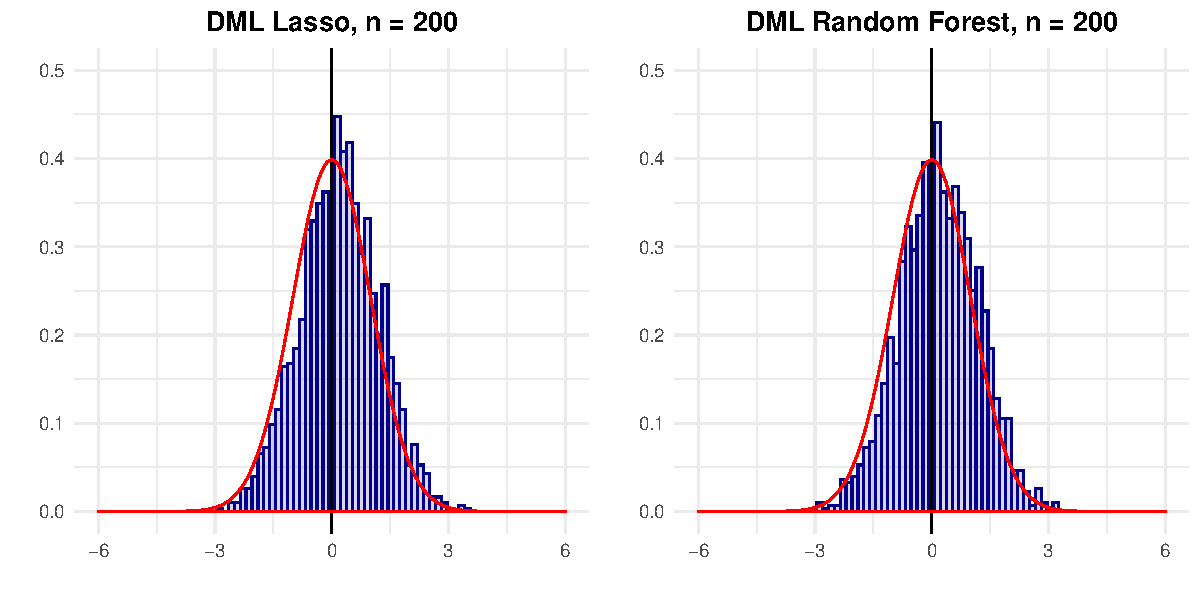
\includegraphics[width=0.8\textwidth]{pictures_and_logos/DMLcomp_dml_resc_n200_p200.pdf}}{ The figure shows two histograms of the empirical distribution (blue bars) of two double machine learning estimators for THETANULL in a simulation example. The estimators are studentized, i.e., the true value of THETANULL is subtracted from the value of the estimator and this difference is then divided by the empirical standard deviation of the simulated estimators. The histogram on the left hand side corresponds to a DML learner that is based on a lasso learner. The histogram on the right hand side corresponds to a DML learner that is based on a random forest. In both figures, the density of a standard normal random variable is illustrated by a red curve, which is symmetric around zero. The empirical distribution of both DML estimators is very similar to the standard normal density which should illustrate the validity of the double machine learning approach.}
\end{center}

\end{frame}
